\chapter{Modulators}
The previous chapters wrote about the audio generators and manipulators. This section will take a look at some usefull modules which are used to modulate parameters within Odin 2. 

Some of the modulators have hardwired functionalities in the synthesizer. However, the true potential of these (and the entire synth, really) lies in appling modulation from the \modmatrix.

\section{ADSR Envelopes}
\label{ADSR}
An ADSR Envelope provides a handy way of setting up a wide variety of curves like they can be observed in the timbre changes of physical instruments. ADSR Envelopes follow two basic signals: MIDI note-on and MIDI note-off. Depending on these, a curve is produced based on the four parameters \fat{Attack, Decay, Sustain} and \fat{Release}.

Odin 2 provides four of these Envelopes:

\begin{center}
    \includegraphics[width=0.4\textwidth]{graphics/ADSR_section.png}
\end{center}

The \fat{Amp Envelope} is hardwired to control the volume curve of the voice. This effect is not applied in the actual Amplifier module, but after the Distortion section (see Section \ref{routing}). Note that the Amp Envelope can still be used as a freely assignable modulation source in the \modmatrix. This Envelope is calculated for each voice independently.
\label{amp_env}

The \fat{Filter Envelope} is hardwired to modulate the frequencies of the various Filter modules in Odin 2. For this to take effect, the parameter "Filter Env" (see Section \ref{filters}) has to be enabled. The modulation by this envelope can be in either positive or negative direction. This Envelope is calculated for each voice independently.

The \fat{Mod Envelope} is a freely assignable modulation source. This Envelope is calculated for each voice independently.

The \fat{Global Envelope} is different from the other three Envelopes in that it exists only once for all voices. This can come in handy when you want the modulation not to diverge between voices.

To switch between the different Envelope modules, use their handles on top of the section:
\begin{center}
    \includegraphics[width=0.5\textwidth]{graphics/ADSR_handles.png}
\end{center}
Two envelopes are paired to occupy the same space. To acces the currently not visible Envelope, simply click on its name.

\begin{center}
    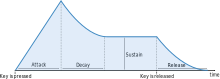
\includegraphics[width=\textwidth]{graphics/ADSR.png}
\end{center}

\audioparameter{Attack}{1}{1}{
    The Attack determines the time the Envelope takes from the start to the first peak. 
    
    When playing the synth in Legato mode (see Section \ref{legato}), the attack section will start from the last value the Enveope from the previous voice produced. No matter the start height, the slope of the Attack will always be the same as if it started from zero.
    
    Using really short Attack times can introduce clicks into the sound, so it is advisable to have at least some attack for most situations.
    
    Note that unlike the Decay and Release sections, the Attack follows a linear curvature.
}

\audioparameter{Decay}{1}{1}{
    The Decay controls the time the Envelope will take to fall to the sustain value after the Attack reached its highest point. This curve will always start at the internal value one, and will always fall to the value specified by the Sustain parameter.

    The Decay section follows an exponential falling curvature.
}

\audioparameter{Sustain}{1}{1}{
    The Sustain determines the level that the Evelope will fall to after the Decay section. Note that the Sustain section will be active after Decay finished for as long as the MIDI-key is not released.
}

\audioparameter{Release}{1}{1}{
    The Release controls the time the Envelope will take to fall to zero after the MIDI-key was released. No matter what stage is currently active, once the key is released, the Envelope will jump right to the Release section immediately. The starting point for the falling curve will always be the last value that the Envelope produced. A finished Release section of the Amp Envelope gives the synthesizer the signal to end processing for this voice.

    The Release section follows an exponential falling curvature.
}

\audioparameter{ADSR Loop}{0}{1}{
    The loop parameter gives the option to start the Attack section again after the Decay is finished, thereby creating an LFO-type modulation source.
}